%!TEX root = ../Thesis.tex
\chapter{Transfer Orbits} \label{ch:transfer orbits}
\epigraph{``\itshape{It's a strange, eerie sensation to fly a lunar landing trajectory—not difficult, but somewhat complex and unforgiving.}"}{--- \textup{Neil Armstrong}}
Transfer orbits is any trajectory of a spacecraft between two different closed orbits, either around the same celestial body or two different bodies. In general, transfer orbits will always be a trade-off between flight time (the total time required for the transfer orbit) and fuel consumption for a specific craft - or equivalently, a trade-off between flight time vs. $\Delta v$ for any craft.

In spacecraft flight dynamics, the change in velocity\footnote{We're really talking about speed here. Velocity and speed are often used interchangeably in orbital mechanics, but fortunately this rarely leads to confusion in practice.} ($\Delta v$ or delta-$v$) is fundamental property of a transfer orbit. The energy- and fuel consumption on the other hand, does depend on the spacecraft. Energy consumption is a practical concern, but not a key part of the underlying physical problem. This is due to the fact that a spacecraft of any mass need the same change in velocity to perform identical orbital maneuvers in a given system of celestial bodies. The basic reason for this is the cancellation of the gravitational mass in Newton's law of universal gravitation and the inertial mass Newton's 2nd law of motion \cite{Knudsen2002}, which are the same by the equivalence principles. Hence
\begin{align}
\vec{F} &= G \dfrac{M m}{r^2} = m \vec{a} \\[0.3cm]
\Leftrightarrow \vec{a} &= \dfrac{G M}{r^2} \vec{\hat{r}} \label{eq:general-eom},
\end{align}
where $G$ is the gravitational constant, $M$ is the larger mass, $m$ is the smaller mass, $r$ is the separation distance between the two masses, $\vec{F}$ is the gravitational force vector from $M$ on $m$ pointing to $M$ along the line connecting their center of masses with unit vector $\vec{\hat{r}}$, and $\vec{a}$ is the acceleration vector of $m$. Thus for any spacecraft of mass $m$, the equation of motion (and hence its trajectory) will be the same independent of the mass $m$, given same initial conditions and that $m \ll M$ so $m$ does not affect the motion of $M$. We can easily generalize to an arbitrary number of large masses $(M_1, M_2 \dots)$. This is all assuming point masses and that the small mass $m$ is sufficiently small as to not affecting the motion of the big masses $(M_1, M_2 \dots)$ significantly. This is the case for spacecrafts in the vicinity of the Earth, whose motion is dominated by the gravitational fields of the Sun, Earth and Moon.

So in planning- and optimizing orbital trajectories, $\Delta v$ is the quantity of interest, a quantity that we may want to optimize along with flight time. Conversely, knowing the mass and fuel capacity of a spacecraft beforehand, determines the so-called $\Delta v$ budget that the spacecraft have at its disposal for various maneuvers.
\\
Before we delve into the different kinds of transfer orbits, we need to introduce some terminology. We imagine a large mass $M$ placed at focus point $F$ and a body of small mass $m$ orbiting it, Figure \ref{fig:ellipse} \cite{Murray1999}. Kepler's first law states that in a 2-body system with a large mass $M$ and a small negligible mass $m$, the orbit of the small body is an ellipse with the large body at one of the foci \cite{Knudsen2002}
\begin{description}
    \item[$F$, $F'$ = Focus] Ellipses have two foci.
    \item[$\vec{r}$ = Position vector of smaller orbiting body.]
    \item[$A$ = Apoapsis] The point on the orbit of greatest distance to the central body\footnote{Also known as the apocentre. If Sun/Earth is central body, also known as aphelion/apogee.}.
    \item[$P$ = Periapsis] The point on the orbit of least distance to the central body\footnote{Also known as the pericentre. If Sun/Earth is central body, also known as perihelion/perigee.}.
    \item[$r_A$ = Distance from central body to apoapsis.]
    \item[$r_P$ = Distance from central body to periapsis.]
    \item[$a$ = Semi-major axis] Half the greatest diameter of the ellipse.
\end{description}

\begin{figure}[ht!]
\centering
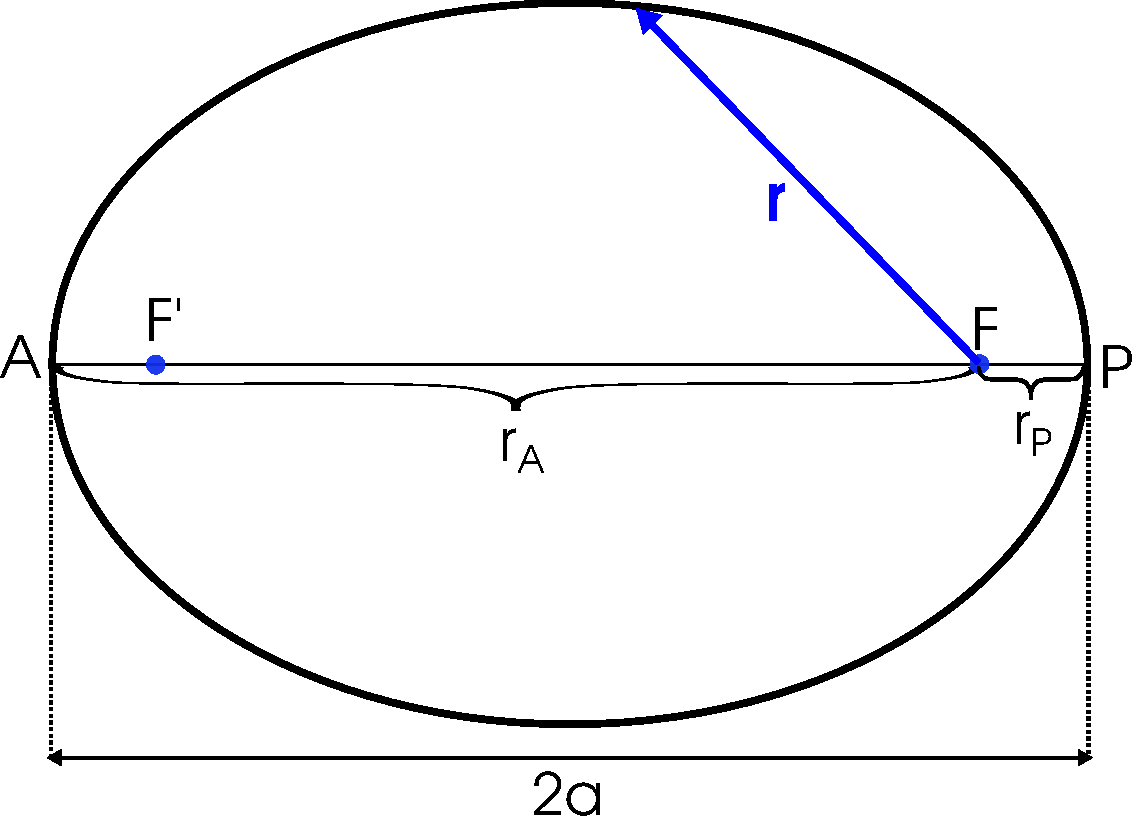
\includegraphics[scale=0.51]{fig/ellipse.pdf}
\caption{The elliptical orbit. See definitions just above figure. Source: \cite{fig-ellipse} (modified)}
\label{fig:ellipse}
\end{figure}


%%%%%%%%%%%%%%%%%%%%%%%%%%%%%%%%%%%%%%%%%%%%%%%%%%%%%%%%%%%%%%%%%%%%%%%%%%%%%%
\section{Hohmann Transfer-Orbit} \label{ch:hohmann}
The Hohmann transfer orbit is an elliptical orbit used to transfer between two circular orbits in the same plane. This is done by doing two engine impulses known as \emph{burns} along the trajectory, see Figure \ref{fig:hohmann}.

\begin{figure}[ht!]
\centering
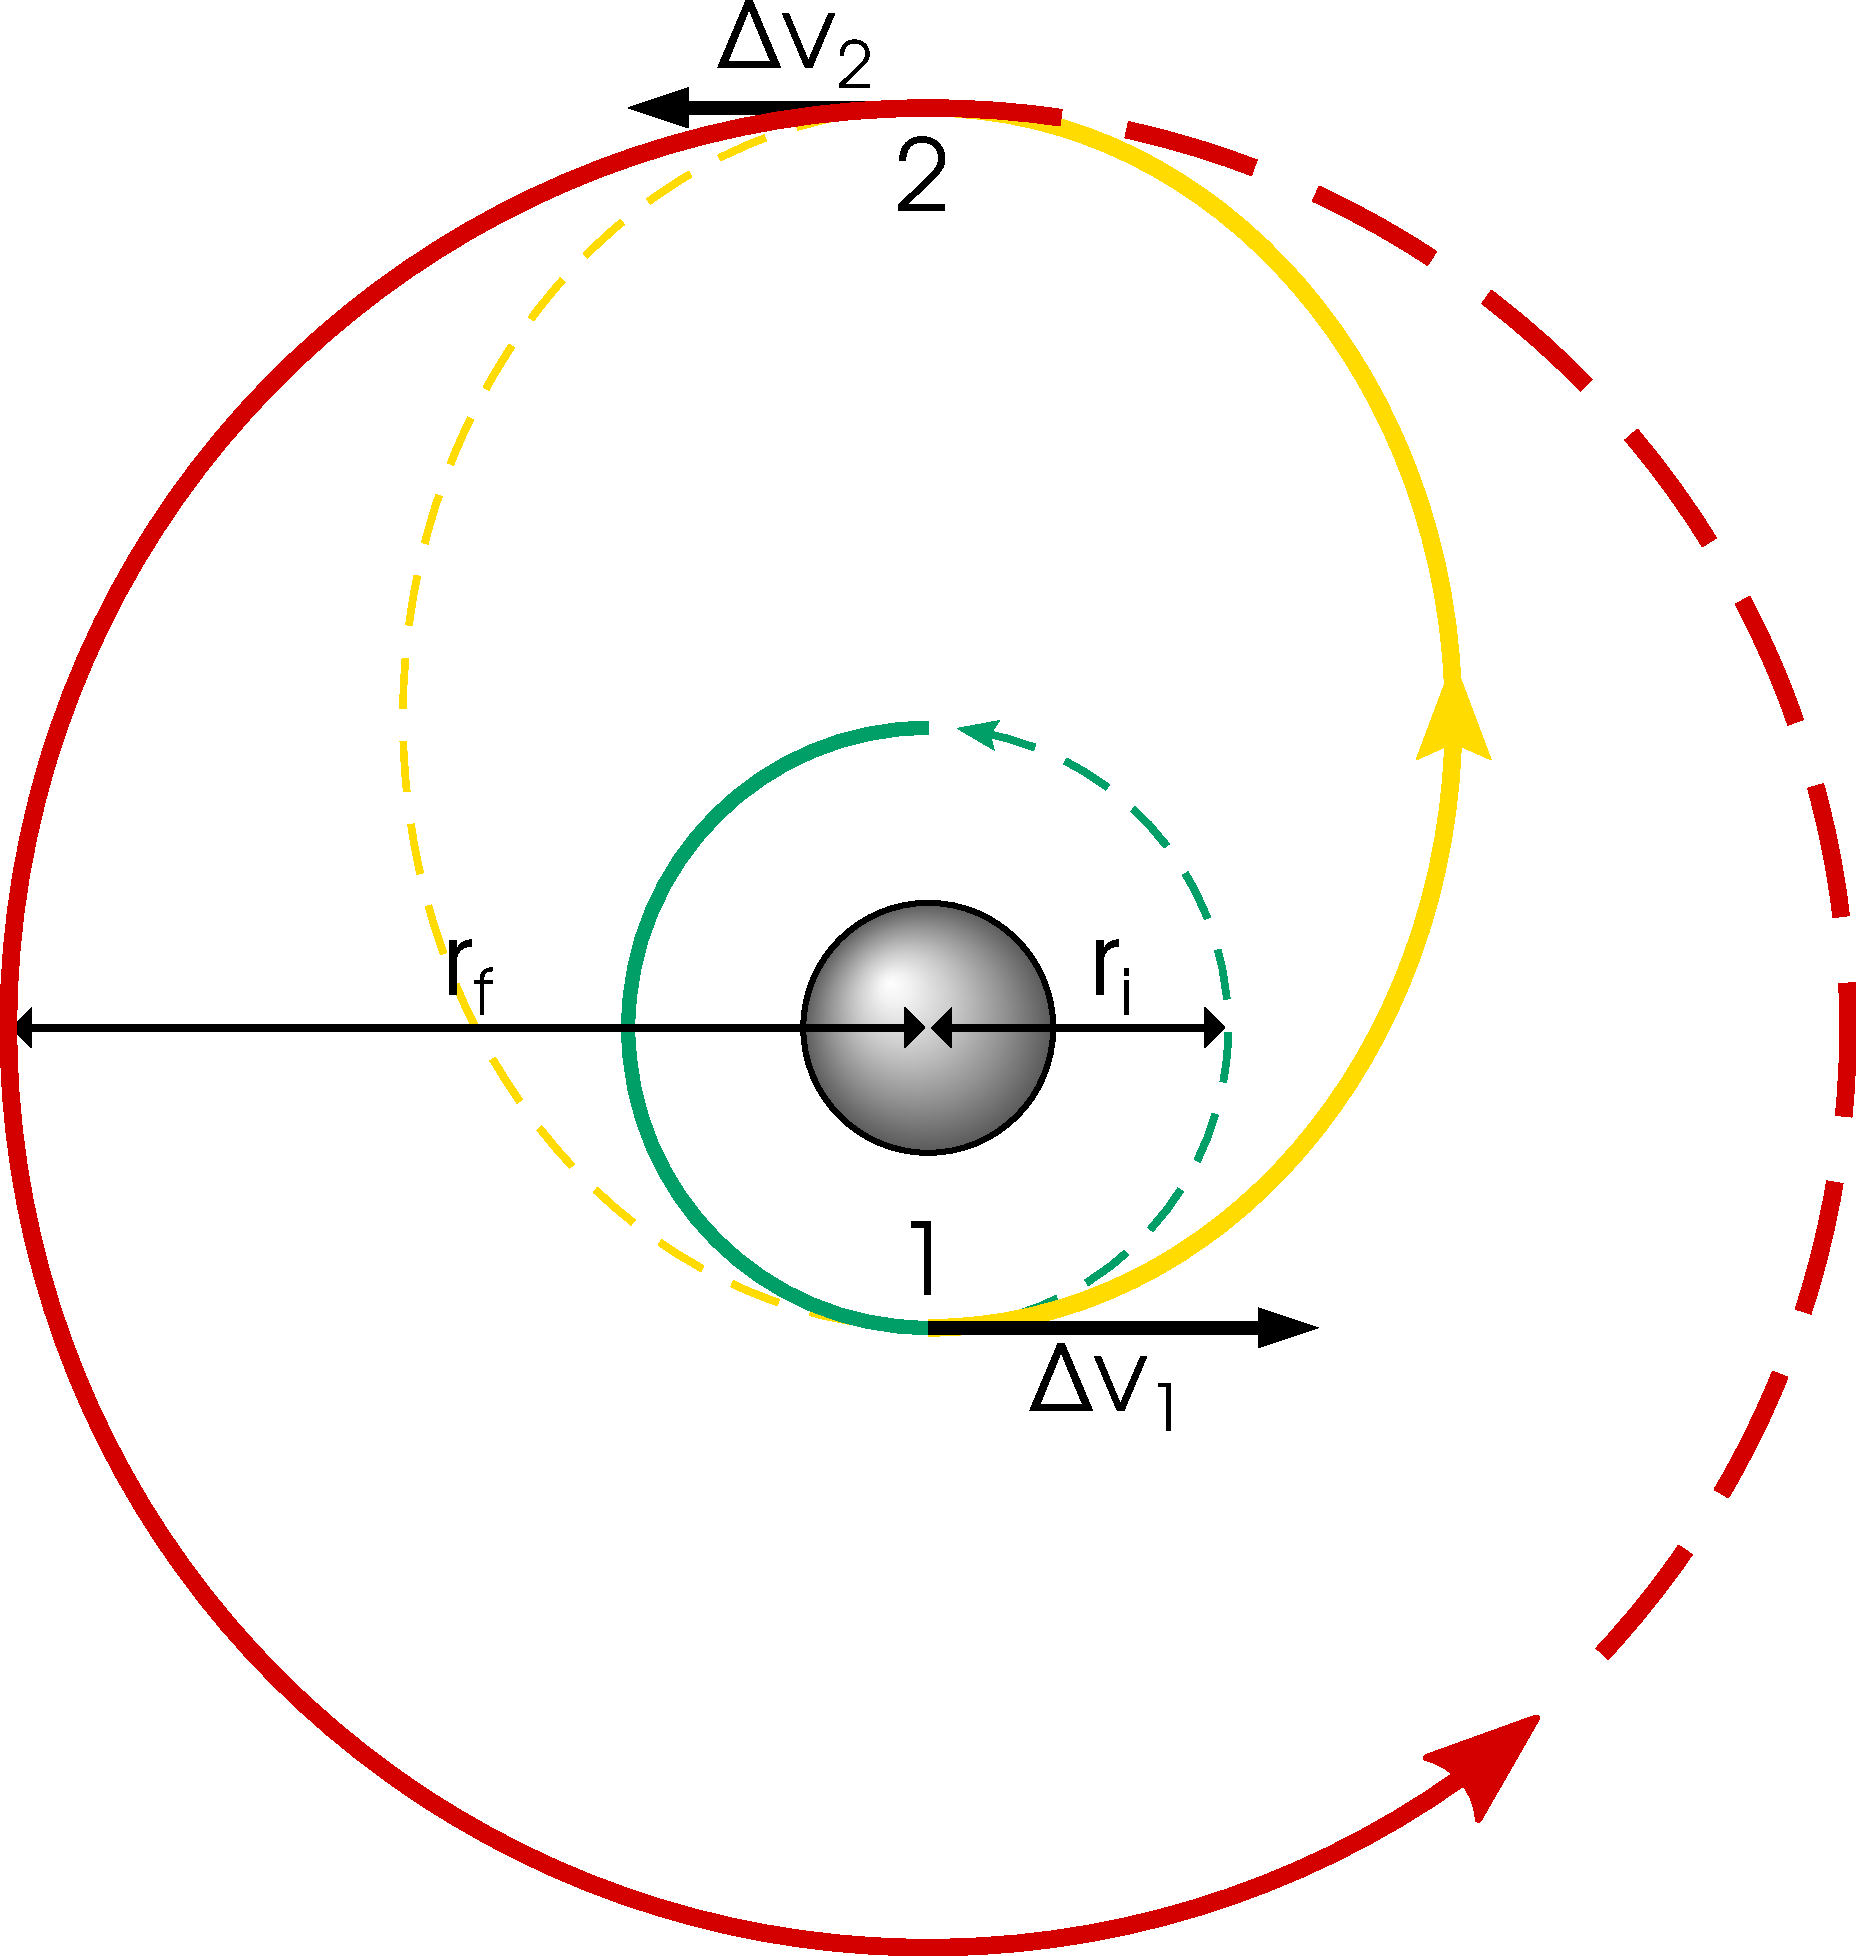
\includegraphics[scale=0.3]{fig/hohmann.pdf}
\caption{The Hohmann transfer orbit. We start in circular orbit around central body at distance $r_i$, 1.) Burn applied prograde (same direction as velocity vector) to change velocity by $\Delta v_1$, now in elliptical orbit around central body, 2.) Another burn is applied prograde at apoapsis to change velocity by $\Delta v_2$, now in circular orbit at distance $r_f$. Source: \cite{fig-hohmann} (modified)}
\label{fig:hohmann}
\end{figure}

All the Apollo missions launched the spacecraft from Earth into a parking orbit around Earth \cite{apollo-parking}\footnote{An intermediate low circular orbit that a spacecraft is placed into temporarily after launch to ensure that all systems are nominal and calculate the precise transfer orbit to the destination}, then a Hohmann-like transfer orbit to the moon, where they achieved circular lunar orbit \SI{99}{\km} above the moon surface. We will assume an initial parking orbit of \SI{160}{\km} above the earth's surface and a capture orbit \SI{100}{\km} above the moon surface.

It has been proved that the Hohmann transfer-orbit is the most $\Delta v$-efficient transfer-orbit from circle-to-circle (or ellipse-to-ellipse) in a 1-body system when $r_f/r_i$ is less than $\approx 11.94$ \cite{Prussing1992} \cite{Peet} \cite{Biesbroek2000}.


%%%%%%%%%%%%%%%%%%%%%%%%%%%%%%%%%%%%%%%%%%%%%%%%%%%%%%%%%%%%%%%%%%%%%%%%%%%%%%
\section{Bi-elliptic Transfer-Orbit}
The bi-elliptic transfer is two elliptical orbits used to transfer between two circular orbits. Thrust is applied at three points instead of Hohmann's two, see Figure \ref{fig:bi-elliptical}. The basic idea is that the first prograde burn will bring the spacecraft close to escape velocity, then at the apoapsis another prograde burn will increase the periapsis distance (see fig \ref{fig:ellipse}) to the desired distance. Finally at periapsis a retrograde (opposite velocity vector) burn will make the orbit circular.

\begin{figure}[ht!]
\centering
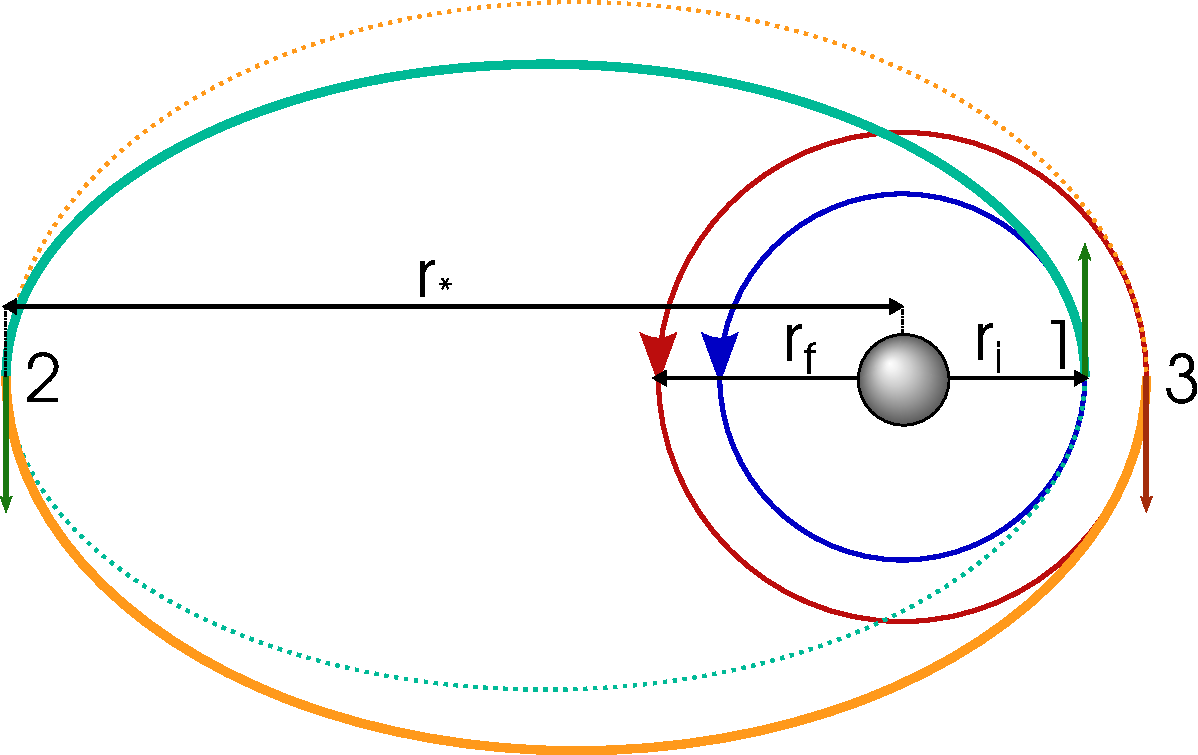
\includegraphics[scale=0.53]{fig/bi-elliptic.pdf}
\caption{The bi-elliptic transfer-orbit. We start in a circular orbit around the central body at distance $r_1$, 1.) Big burn applied prograde to change velocity close to escape velocity, now in arbitrarily big elliptical orbit with $r_*$ as apoapsis distance, 2.) Small burn applied prograde at apoapsis to increase periapsis distance from $r_i$ to desired $r_f$, 3.) Small burn applied retrograde at periapsis to decrease apoapsis distance from $r_*$ to $r_f$, now in circular orbit at distance $r_f$. Source: \cite{fig-bi-elliptical} (modified)}
\label{fig:bi-elliptical}
\end{figure}
It has been proven that the bi-elliptic transfer-orbit is the most $\Delta v$-efficient transfer-orbit from circle-to-circle (or ellipse-to-ellipse) in a 1-body system when $r_f/r_i$ is greater than $\approx 11.94$ \cite{Prussing1992} \cite{Peet}. We will not consider the bi-elliptic to the Moon. The reason for this is outlined below.

In our case $r_i = \SI{160}{\km}$ (Earth parking orbit) and $r_f = \SI{3.85e5}{\km}$ so
\begin{align}
r_f/r_i = \dfrac{\SI{3.85e5}{\km}}{\SI{6367}{\km}+\SI{160}{\km}} \approx 59.0
\end{align}
The closer the velocity is to escape velocity right after the first burn at point in fig \ref{fig:bi-elliptical}, the greater the apoapsis distance $r_*$ will be, going to infinity at escape velocity. As $r_*$ increases, the flight time tends to infinity and the bi-elliptic orbit gets more efficient. Note that the $\Delta v$ of the Hohmann- and the bi-elliptic transfers converges to the same value in the limit as $r_f/r_i \to \infty$ see Figure \ref{fig:hohmann_vs_bi-elliptic1}. Also note the local minimum of the ratio $\Delta v_{\text{Bi-elliptic}}/\Delta v_{\text{Hohmann}}$ at $r_f/r_i = 57.19$, which is very close to the moon trip of 59.0 (caveat: $r_*$ is set to $\infty$). This means that the bi-elliptic transfer should theoretically even be most beneficial compared to Hohmann at the moon distance. Even so, we will not consider the bi-elliptic to the Moon.
\begin{figure}[ht]
\centering
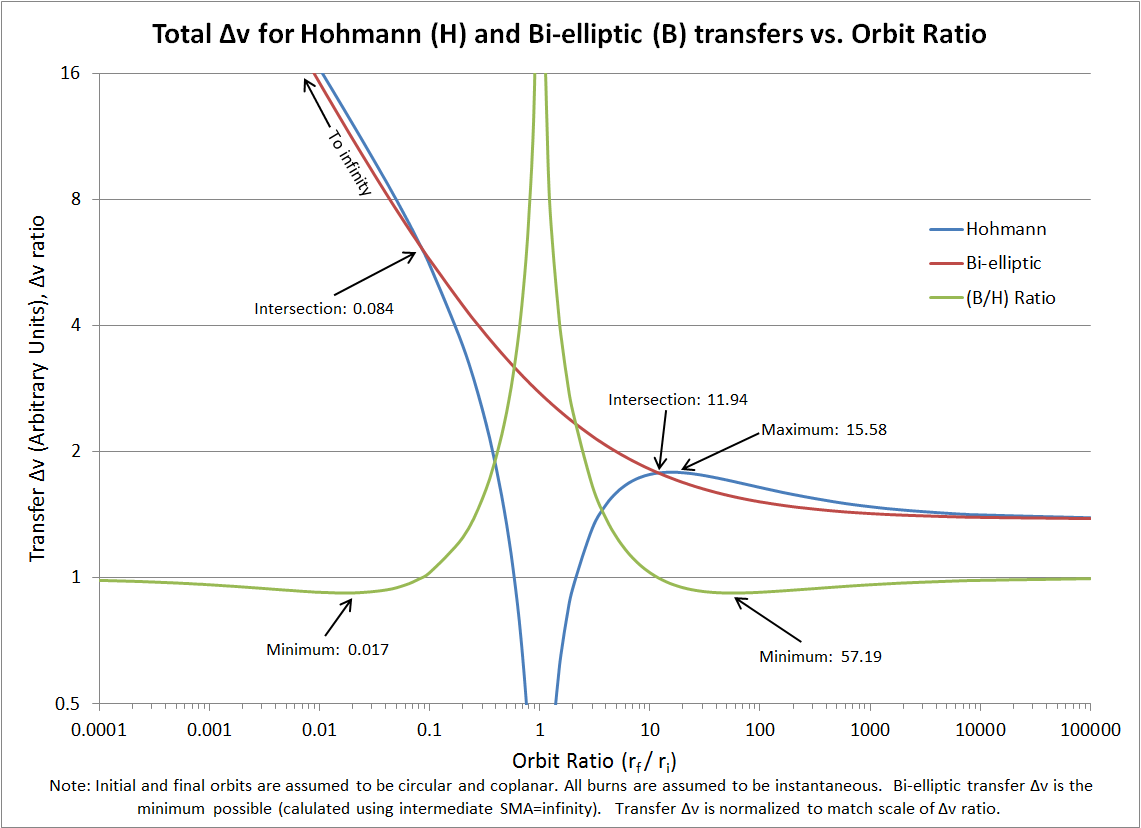
\includegraphics[scale=.47]{fig/hohmann_vs_bi-elliptic1.png}
\caption{$\Delta v$ as a function of the orbit ratio $r_f/r_i$ for Hohmann and bi-elliptical transfer orbits. $r_i$ is initial orbit distance, $r_f$ is final orbit distance. They intersect at $r_f/r_i \approx 11.94$, where bi-elliptical becomes more efficient than Hohmann, but they converge as $r_f/r_i \to \infty$. This is best case for bi-elliptic since we have set $r_*=\infty$. Source:\cite{Copperheadtnp}}.
\label{fig:hohmann_vs_bi-elliptic1}
\end{figure}
Figure \ref{fig:hohmann_vs_bi-elliptic2} shows effiencies for various intermediate orbital radii $r_*$.
\begin{figure}[ht]
\centering
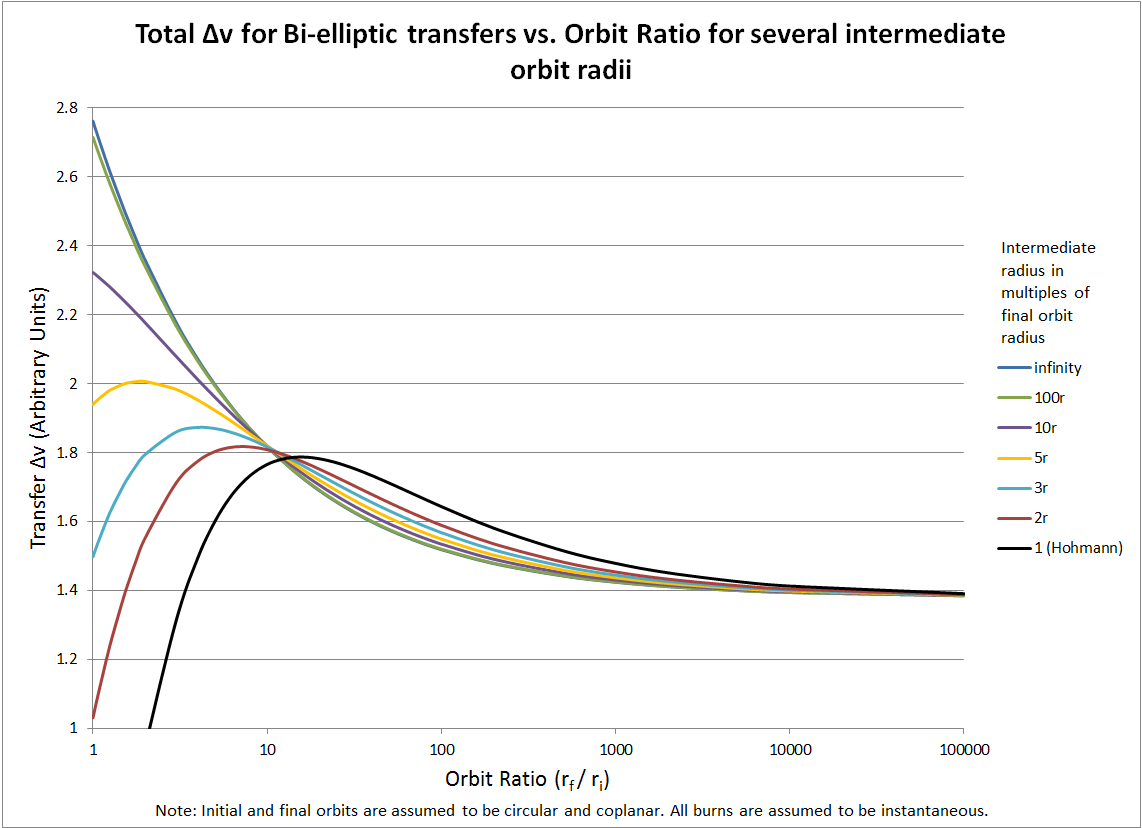
\includegraphics[scale=.47]{fig/hohmann_vs_bi-elliptic2.png}
\caption{$\Delta v$ for various intermediate orbit apoapsis radii $r*$ as function of the ratio $r_f/r_i$, where $r_i$ is the initial orbit distance and $r_f$ is the final orbit distance. Once gain we see the intersect at $r_f/r_i = 11.94$, where bi-elliptical becomes more efficient than Hohmann, the two of them converge as $r_f/r_i \to \infty$. Source: \cite{Copperheadtnp}}
\label{fig:hohmann_vs_bi-elliptic2}
\end{figure}
To take advantage of the bi-elliptic transfer, we must make $r_*$ as large as possible. This is not achievable in practice due to both very long flight times and perturbations from other bodies. As an example, going from LEO at altitude \SI{330}{\km} to $1.3$ times the distance to the moon, requires \SI{99.0}{\percent} of the Hohmann $\Delta v$ \cite{wiki-bi-elliptic}. So it quickly becomes a big trade-off in flight time to save just a little $\Delta v$. While bi-elliptic transfers are considered more complicated, risky and not worth the flight time trade-off for bigger transfers, and therefore are rarely used for that \cite[p. 78]{Taylor2009}, they are often used when performing small, $0 < r_f/r_i < 1$ maneuvers\footnote{Soyuz capsules heading for ISS \cite{esa-soyuz}, launched from Earth into parking orbit use bi-elliptic transfers to dock with ISS. The mid-burn gives opportunity to correct the trajectory. And safety is of great concern for a \$100 billion space station \cite{iss-worth}.}.


%%%%%%%%%%%%%%%%%%%%%%%%%%%%%%%%%%%%%%%%%%%%%%%%%%%%%%%%%%%%%%%%%%%%%%%%%%%%%%
\section{Hohmann-Approximated Transfer-Orbit to the Moon} \label{ch:hohmann-moon}
We will now apply the Hohmann transfer orbit, a model for a 1-body system, as an approximation to find a transfer orbit to the moon, with the Earth-Moon system being a 2-body system. We work on the assumptions:
\begin{description}
    \item[1. Sun is neglected.] The gravitational pull from the sun is neglected. It is not insignificant compared to the earth and the moon, but it's a first-order effect. As long as we do not get too far away from the Earth-Moon system, it should not be a problem.
    \item[2. Moon orbit assumed circular and co-planar with the earth] We assume orbital eccentricity $e = 0$ (perfect circle) and inclination angle (angle between orbital planes of the moon and Earth) $\phi = 0$. These assumptions are reasonable, since the true values are $e = 0.0549$ and $\phi = 5.16 \degree$ \cite{ma}. This assumption reduces the problem from 3 to 2 dimensions, greatly simplifies all equations and does not affect the qualitative conclusions.
    \item[3. Spacecraft does not affect Earth or Moon] The mass of the spacecraft itself is so small that it does not affect the motions of the earth and the moon. With this assumption the three-body problem is called \emph{restricted}, and the Hohmann can be done analytically.
    \item[4. Hohmann can approximate a trans-lunar injection + lunar orbit insertion] A trans-lunar injection (TLI) is a propulsive maneuver used to set a spacecraft on a trajectory that will cause it to arrive at the moon \cite{NASA1966}. We assume that a Hohmann transfer, modified to end with a velocity that matches the centripetal velocity required for circular motion around the moon, is an adequate model. Hence we neglect the gravitational attraction from the moon on the spacecraft while it is in transit, up until the point when the spacecraft is in the circular orbit around the moon.
\end{description}

Our Hohmann transfer orbit to the moon follows the same steps as the standard Hohmann transfer described in chapter \ref{ch:hohmann}, except we end with a slightly different velocity to match a circular orbit centered around the moon, see Figure \ref{fig:hohmann-moon}. In fact we will see that we need to break (retrograde burn) instead of accelerating to achieve desired speed for orbit around the moon rather than around the former central body, the Earth.

\begin{figure}[ht!]
\centering
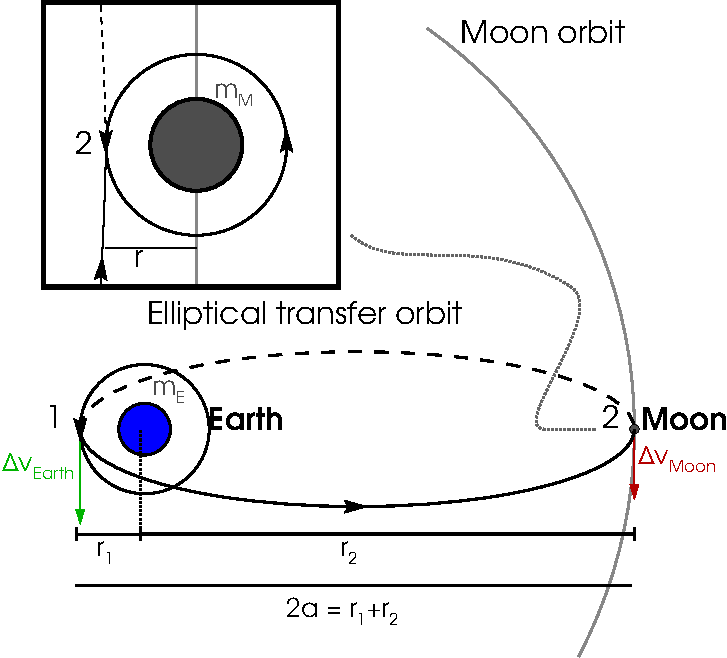
\includegraphics[scale=1.04]{fig/hohmann_moon2.pdf}
\caption{A direct transfer orbit to the moon approximated by Hohmann transfer-orbit. $m_E$ is the mass of the earth, $m_M$ is the mass of the moon. We start in circular orbit around the earth at distance $r_1$ with velocity $v_{\text{earth}}$ 1.) Burn applied prograde to change velocity by $\Delta v_{\text{earth}}$, now in elliptical orbit around the earth with $r_2$ as apogee distance, 2.) Smaller burn applied retrograde at apogee to match a circular orbit around the moon at distance $r_3$ to Moon and velocity $v_{\text{moon}}$ in Moon-system.}
\label{fig:hohmann-moon}
\end{figure}

First we need the \emph{vis viva} equation \cite{Pisacane2005}, which is basically energy conservation applied to elliptical orbits. It serves to relate the distance between two bodies and orbital speed in any Keplerian orbit (elliptic, parabolic, hyperbolic, or radial). We will be using it in the elliptical case:
\begin{align}
v^2 = \mu \left(\dfrac{2}{r} - \dfrac{1}{a} \right) \label{eq:vis-viva} ,
\end{align}
where $v$ is the velocity of the smaller body relative to the central body, $\mu=G M$ is the standard gravitational parameter, $M$ is the central body mass, $r$ is distance from Earth (at focus point) to spacecraft and $a$ is the semi-major axis, see Figure \ref{fig:hohmann-moon}.

Using Figure \ref{fig:hohmann-moon} as reference, we will calculate the total $\Delta v$ to perform a Hohmann transfer orbit from a \SI{160}{\km} circular orbit around the earth to a \SI{100}{\km} circular orbit around the moon. We have the quantities \cite{ma}
\begin{align}
\mu_E &= G m_E = \SI[per-mode=fraction]{6.67e-11}{\m\cubed\per\kg\per\s\squared} \cdot \SI{5.97e24}{\kg} = \SI{3.99e5}{\km\cubed\per\s\squared}, \\[0.2cm]
\mu_M &= G m_M = \SI[per-mode=fraction]{6.67e-11}{\m\cubed\per\kg\per\s\squared} \cdot \SI{7.35e22}{\kg} = \SI{4.90e3}{\km\cubed\per\s\squared}, \\[0.2cm]
r_1 &= \text{Earth radius} + \SI{160}{\km} = \SI{6367}{\km}+ \SI{160}{\km} = \SI{6527}{\km}, \\[0.2cm]
r_2 &= \text{average Earth-Moon distance} = \SI{3.85e5}{\km}, \\[0.2cm]
r_3 &= \text{Moon radius} + \SI{100}{\km} = \SI{1738}{\km}+ \SI{160}{\km} = \SI{1838}{\km}.
\end{align}
All the following $\Delta v$ impulse calculations use the vis-viva equation \eqref{eq:vis-viva} with various values for $r$ and $a$ and velocities are in the geocentric system unless otherwise specified.

\subsection{Impulse at Earth}
Velocity in circular Earth orbit at distance $r_1$ ($r = r_1,\ a = r_1$):
\begin{align}
v_{\text{earth}} = \sqrt{\mu_E\left(\dfrac{2}{r_1} - \dfrac{1}{r_1}\right)} = \sqrt{\dfrac{\mu_E}{r_1}} = \SI{7.814}{\km\per\s}. \label{eq:v-earth}
\end{align}
Velocity in elliptical Earth orbit at perigee distance $r_1$ ($r = r_1,\ a = (r_1+r_2)/2$):
\begin{align}
v_p = \sqrt{\mu_E\left(\dfrac{2}{r_1} - \dfrac{1}{\frac{r_1+r_2}{2}}\right)} = \sqrt{\dfrac{\mu_E}{r_1} \dfrac{2 r_2}{r_1+r_2}} = \SI{10.96}{\km\per\s}, \label{eq:vp}
\end{align}
so the necessary delta-$v$ at Earth:
\begin{align}
\Delta v_{\text{earth}} = v_p - v_{\text{earth}} = \SI{3.144}{\km\per\s}. \label{eq:deltav-earth}
\end{align}

\subsection{Impulse at Moon orbit - ignoring the moon}
Velocity in elliptical Earth orbit at apogee distance $r_2$ ($r = r_2,\ a = (r_1+r_2)/2$):
\begin{align}
v_a = \sqrt{\mu_E\left(\dfrac{2}{r_2} - \dfrac{1}{\frac{r_1+r_2}{2}}\right)} = \sqrt{\dfrac{\mu_E}{r_2} \dfrac{2 r_1}{r_1+r_2}} = \SI{0.1858}{\km\per\s}. \label{eq:va}
\end{align}
Velocity in circular Earth orbit at distance $r_2$ ($r = r_2,\ a = r_2$):
\begin{align}
v_{\text{earth2}} = \sqrt{\dfrac{\mu_E}{r_2}} = \SI{1.017}{\km\per\s},
\end{align}
so the necessary $\Delta v$ at Moon orbit to enter circular Earth orbit (if the moon was not there) is an increase in velocity of
\begin{align}
\Delta v_{\text{no-moon}} = v_{\text{earth2}} - v_a = \SI{0.832}{\km\per\s}.
\end{align}

\subsection{Impulse at Moon orbit - including the moon}
However we can't follow the moon stationary along its orbit, we need to go into a circular orbit around the moon, so we'll make a correction to our $\Delta v_{\text{no-moon}}$.\\
\\
Velocity in circular orbit at distance $\SI{100}{\km}$ above the moon surface \emph{in Moon system}:
\begin{align}
v_{\text{moon}} = \sqrt{\dfrac{\mu_M}{r_3}} = \SI{1.633}{\km\per\s}.
\end{align}
Now we can choose to add or subtract this value to $\Delta v_{\text{no-moon}}$ since we can go into orbit both ways around the moon (clockwise and counterclockwise). We will subtract $v_{\text{moon}}$ from $\Delta v_{\text{no-moon}}$ since this minimizes the $\Delta v$.

So the necessary change in velocity needed to go from geocentric elliptical orbit to circular Moon orbit is a decrease in velocity:
\begin{align}
\Delta v_{\text{moon}} = \Delta v_{\text{no-moon}} - v_{\text{moon}} = \SI{-0.8017}{\km\per\s}, \label{eq:deltav-moon}
\end{align}
so the total $\Delta v$ for the whole trip is
\begin{align}
\Delta v_{\text{total}} = |\Delta v_{\text{earth}}| + |\Delta v_{\text{moon}}| = \SI{3.946}{\km\per\s}. \label{eq:hohmann-delta-v}
\end{align}
The flight time is approximately the time spend on the elliptical orbit, which is half the elliptical orbital period, so by Kepler's third law \cite{Murray1999}:
\begin{align}
t_{\text{Hohmann}} = \dfrac{1}{2}\sqrt{\dfrac{4\pi^2 (\frac{r1+r2}{2})^3}{\mu_E}} = \SI{5.0}{\days}. \label{eq:hohmann-flight-time}
\end{align}
A more detailed analysis of a Hohmann-like LTI with identical initial and final orbits, turns out a very similar $\Delta v_{\text{total}} = \SI{3.959}{\km}$ \cite{Sweetser1991} \cite{Juul2008}. This seems to somewhat justify our fourth and perhaps seemingly most questionable assumption at the beginning of the section.

Coincidentally our $\Delta v_{\text{total}}$ in \ref{eq:hohmann-delta-v} is actually pretty close to the moon-less scenario:
\begin{align}
\Delta v_{\text{total-no-moon}} = |\Delta v_{\text{earth}}| + |\Delta v_{\text{no-moon}}| = \SI{3.976}{\km\per\s}.
\end{align}
This makes it relevant to pose the question: could we possibly minimize $\Delta v_{\text{total}}$ by choosing a moon orbit altitude such that the necessary moon orbiting velocity in the moon system is equal to the incoming velocity on the ellipse at the intersection in the Earth system? In effect, meaning no velocity change necessary at point 2 in fig \ref{fig:hohmann-moon}, i.e. $\Delta v_{\text{moon}} = 0$? We set $r_3 = \text{Moon radius} + x$ and solve $\Delta v_B = 0$ for $x$ and find $x = \SI{5350}{\km}$ and $\Delta v_\text{total-min} = \SI{3.144}{\km\per\second}$ (see Appendix \ref{app:hohmann-moon} for calculations and $\Delta v_\text{total}$ vs. Moon orbital distance plot). This is a valid orbital altitude since its well within the moon's Hill sphere of radius of roughly \SI{62,000}{\km}. The Hill sphere radius marks the point between Earth and Moon at which a spacecraft switches from orbiting one to orbiting the other, measured from Moon (the smaller body). In more precise terms the Hill sphere is the approximate equipotential surface around a smaller body $m$ orbiting a larger body $M$ at distance $r_{m,M}$, indicating the boundary of the region where a smaller spacecraft $m_s$ would orbit $m$ rather than $M$. In other words its the distance from $m$ where the forces from $M$ and $m$ add up to the centripetal force towards $M$. The radius of the Hill sphere is given by \cite{Murray1999}
\begin{align}
r_{\text{hill}} = r_{m,M}\sqrt[3]{\dfrac{m}{3M}}. \label{eq:hill-sphere}
\end{align}
The Hill sphere of the moon in our Earth-Moon system is (appendix \ref{app:hohmann-moon}):
\begin{align}
r_{\text{hill-moon}} = r_2\sqrt[3]{\dfrac{m_M}{3m_E}} = 0.16 r_2 = \SI{62,000}{\km}.
\end{align}

So the Hohmann transfer orbit is the most effective way of getting into a high lunar orbit. It is also the fastest way to the moon. The Apollo missions used \SI{4.115}{\km\per\s} and took 3.05 days. However ultimately we're not just interested in getting in \emph{any} circular orbit around the moon, but in low lunar orbit (LLO) (lunar orbits less than \SI{100}{\km} altitude \cite{NASA1966}) at low $\Delta v$ for the purpose of unmanned orbital missions- or landings.\\
\\
Now that we fully understand the Hohmann-like TLI, its performance and limitations, we're ready to look at the low-energy transfer orbits.


%%%%%%%%%%%%%%%%%%%%%%%%%%%%%%%%%%%%%%%%%%%%%%%%%%%%%%%%%%%%%%%%%%%%%%%%%%%%%%
\section{Low-Energy Transfer Orbits - Slow But Cost-Effective}
In 1990 the Japanese spacecraft ``Hiten'' was launched and failed part of its mission, ending in a high elliptical around the Earth, however with insufficient fuel to perform the Hohmann transfer-orbit maneuver to reach the Moon. Edward Belbruno proposed an non-traditional trajectory that could get the spacecraft to the Moon anyway \cite{universe-today-hiten}. Originally invented by Belbruno in 1987 \cite{Seefelder2002}, this marked the first practical use of a \emph{low-energy transfer orbit} \cite{nasa-hiten}, that is an orbit that uses little fuel compared to traditional direct-route transfer-orbit such as Hohmann. Figure \ref{fig:hiten} shows the mission trajectory profile. It was a success and marked the beginning of an active research area in low-energy transfer orbits, also known as weak stability boundary trajectories or ballistic capture trajectories.

\begin{figure}[ht!]
\centering
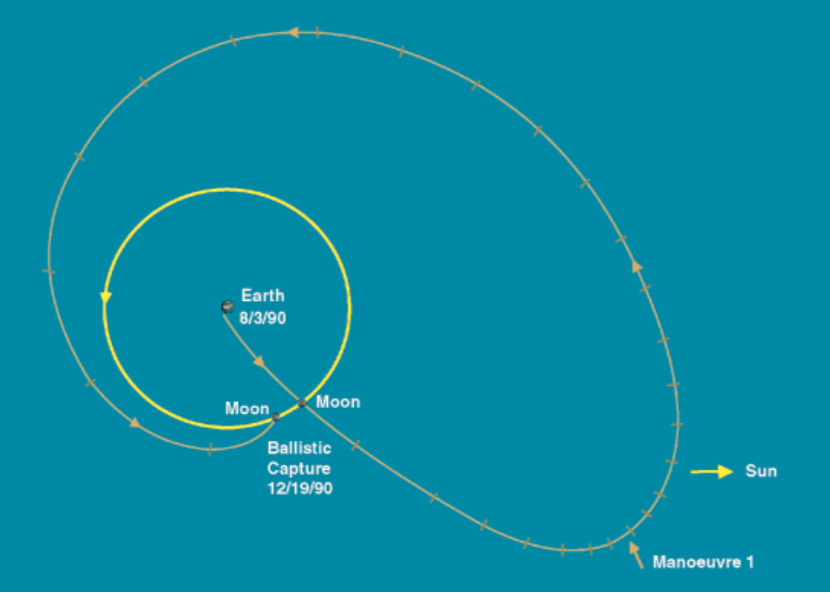
\includegraphics[scale=0.8]{fig/hiten.png}
\caption{Hiten mission profile showing the Belbruno trajectory, which interacts with the moon twice in order to be captured ballistically by the moon. Tick marks are at 5 day intervals. Source: \cite{Biesbroek2000}}
\label{fig:hiten}
\end{figure}

In the last section we found that Hohmann transfer orbits to the moon need to brake at the moon to shed $\SI{0.832}{\km\per\s}$. The idea of a low-energy transfer-orbit is to have the spacecraft captured ballistically by the moon, spending much less fuel on firing retrorockets when the spacecraft reaches the moon. We can expect savings in $\Delta v$ up to $\SI{150}{\m\per\s}$ at the expense of the flight time going from the order of 5 days to 60-100 days \cite{Garcia2007}. A saving of \SI{150}{\m\per\s} is a small proportion of the total delta-$v$, but since the $\Delta v$ and fuel are being saved from a late point in the trip (braking at the moon), it takes a lot of fuel to transport the fuel itself to the moon and the effect is quite significant: upwards of \SI{25}{\percent} can be saved off the $\Delta v$ after leaving LEO. As a result under some circumstances, double the payload mass that can be placed into LLO (Low Lunar Orbit) \cite{Belbruno2000}.

Another advantage is more flexible launch windows. A launch window is the time intervals during which the launch of a particular mission is possible from a specific location. Launch windows vary in both size and frequency. During the Apollo missions, the monthly launch window consisted of a few days during a given month or lunar cycle. The daily window had a duration of a few hours during a given 24 hour period \cite{nasa-apollo-launch-window}. Since a low-energy transfer-orbit can approach it's target from many more directions due to it's chaotic nature, they provide more flexibility concerning launch time windows compared to the more traditional Hohmann transfers. It has been demonstrated that it is possible to achieve lunar orbit for a 20 minute launch window on a given day for only up to about 50 m/s $\Delta v$ extra. Furthermore, for an additional 50 m/s a launch period of about 5 days per lunar cycle can be achieved \cite{Belbruno2000}.

The flexibility advantage is even more pronounced for Mars, where three advantages can be highlighted: the $\Delta v$ performance, the much more flexible launch windows (Hohmann to Mars is just a few times a year), and finally that it is safer than Hohmann in the sense that the capture $\Delta v$ is applied far from Mars and in a gradual manner.  By comparison, the capture process for a Hohmann transfer needs to be done very quickly and be precisely timed or the spacecraft is lost. \cite{Topputo2014}.

In any optimization scheme is it very useful to know the theoretical limit. For a trajectory that starts in a circular orbit $\SI{167}{\km}$ above the Earth orbit and ends at a $\SI{100}{\km}$ altitude circular polar moon orbit, \cite{Sweetser1991} found a lower bound of $\Delta v$ at \SI{3.721}{\km\per\s}. The associated trajectory does not exist since it requires, theoretically, an infinite time to approach $L_1$ and to depart from it \cite{Topputo2005}.

Even in the simplest model, the planar circular restricted three-body problem that we have chosen, the system is chaotic. Therefore the low-energy transfer orbits cannot be found analytically and we must apply some trial-and-error to find them. However instead of relying completely on brute force, randomly searching through all possible trajectories, we can be guided by theory some of the way by studying the energy contours of the system. To this end it is useful to introduce Lagrange points.

\subsection{Lagrange Points and Low-Energy Transfer Orbits}
For two large bodies of masses $M$ and $m$ there exists points in space where the sum of the gravitational forces from the two bodies equals the centripetal force required to orbit with them around the center of mass \cite{Murray1999}. There exists five such points denoted by $L_1 - L_5$, see Figure \ref{fig:lagrange-points}.

\begin{figure}[ht]
\centering
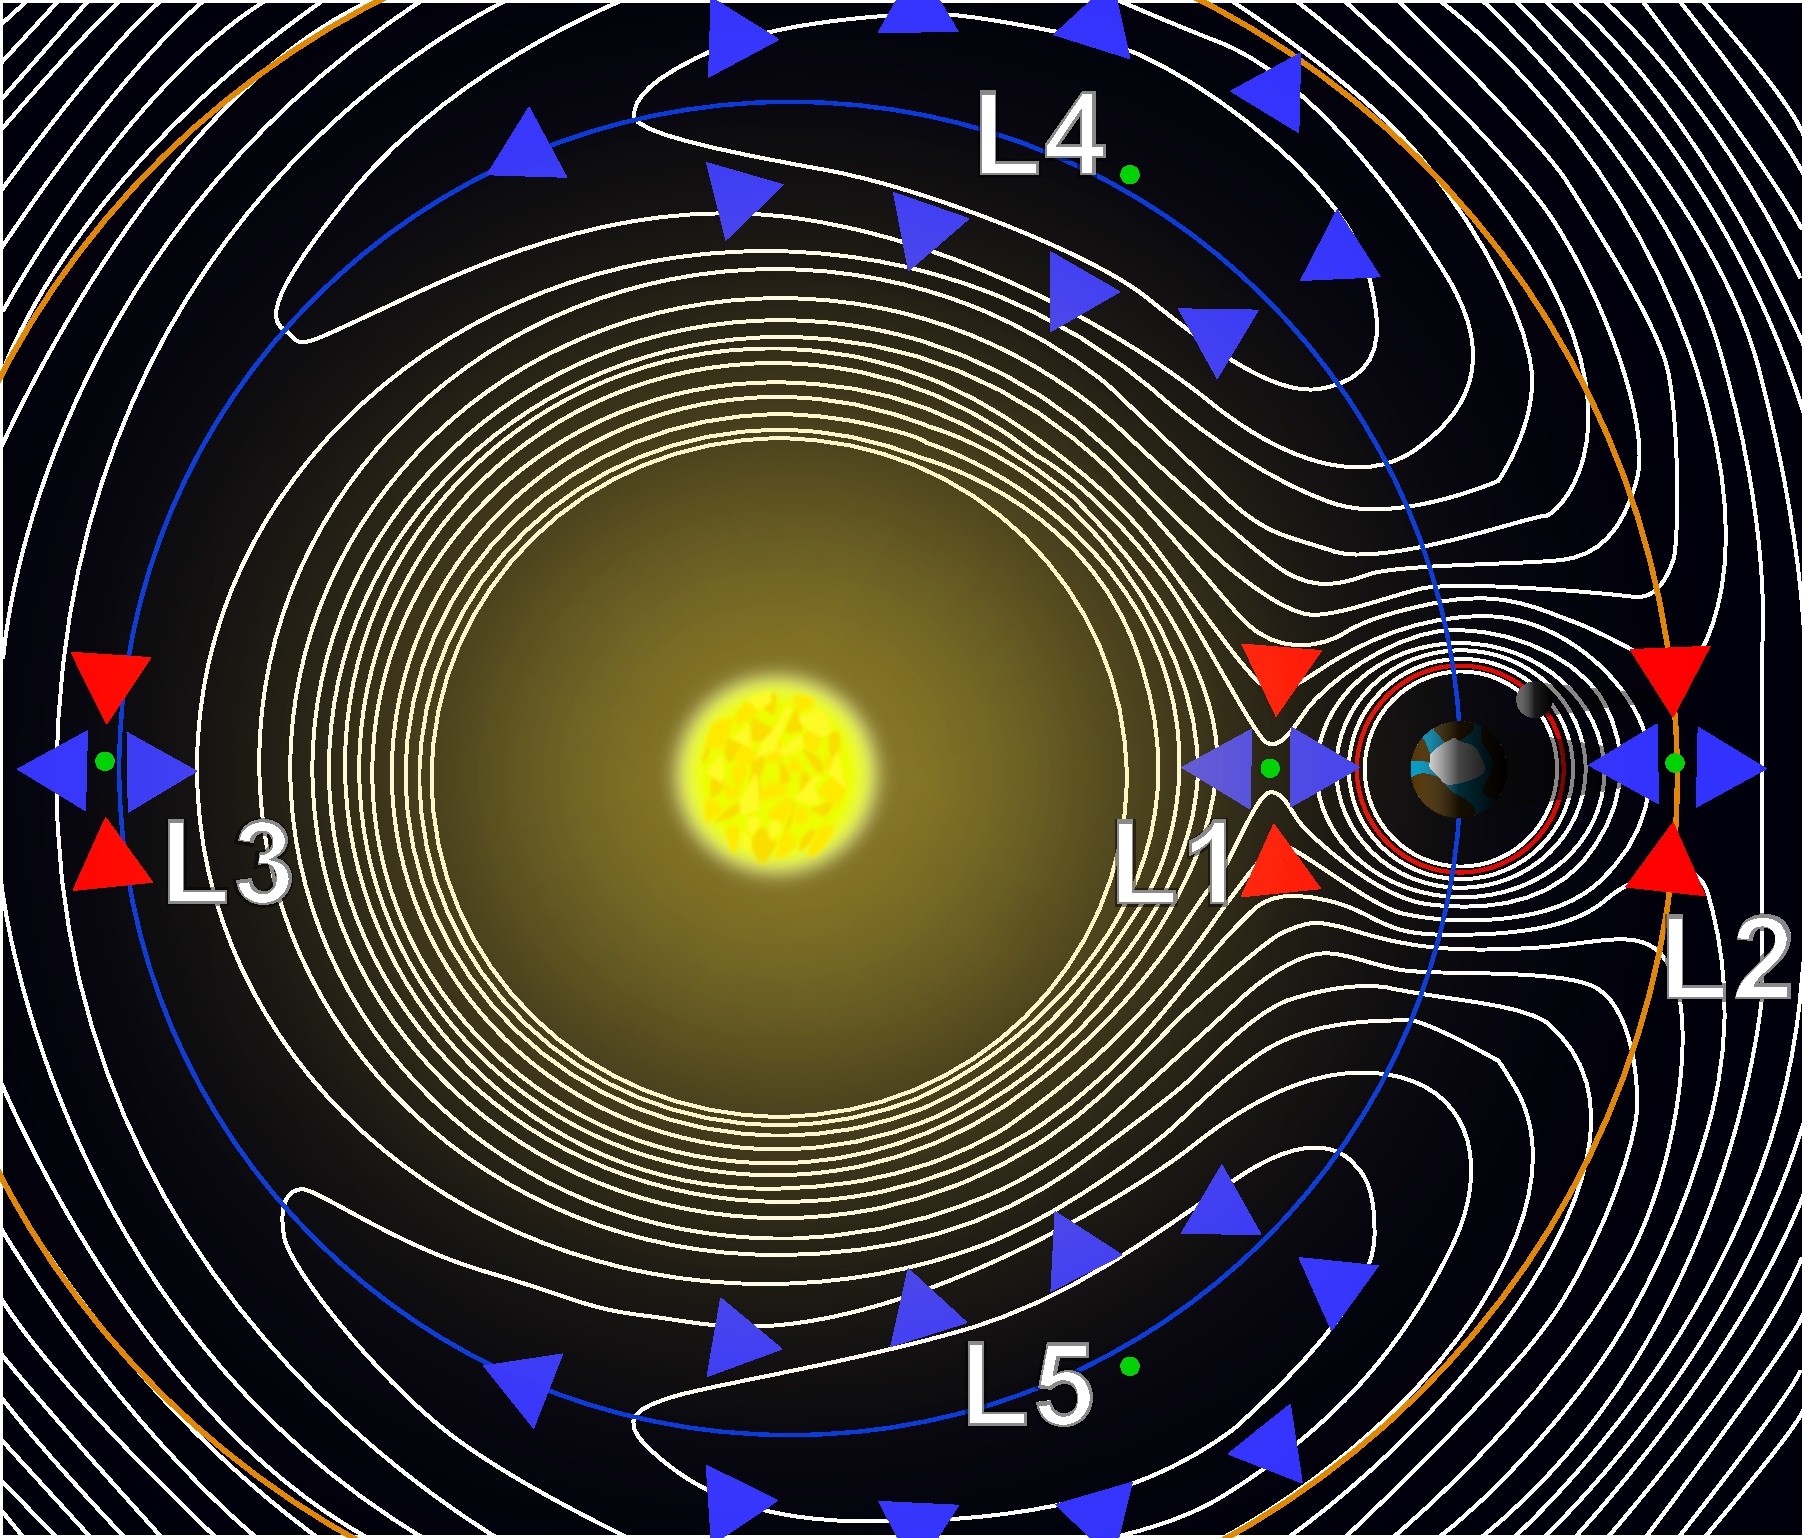
\includegraphics[scale=0.32]{fig/lagrange_points.pdf}
\caption{Contour plot of the effective potential due to gravity of a two-body system in a rotating frame of reference. The red and blue arrows indicate positive and negative potential gradients, respectively. Also shows all the Lagrange Points $L_1-L_5$ are indicated by green dots. They are points of equilibria, or stationary points where the all the gravitational forces and centrifugal force cancel out. Note that this picture depicts the potential and Lagrange points of Sun-Earth (the moon is only there for show) but it applies equally well the Earth-Moon or any other 2-body system}
\label{fig:lagrange-points}
\end{figure}

If $M \gg m$, then the distance to $L_1$ and $L_2$ from $m$ are exactly equal to the Hill sphere \eqref{eq:hill-sphere}.

\begin{figure}[ht]
    \centering
        \subbottom[Effective potential]{
            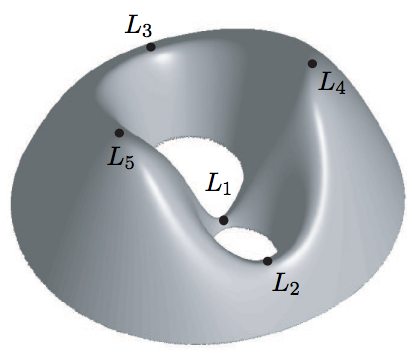
\includegraphics[scale=0.80]{fig/2bp-a_effective-potential.png}
            \label{fig:effective-potential}
        }
        \subbottom[Equipotential slice, allowed and forbidden regions]{
            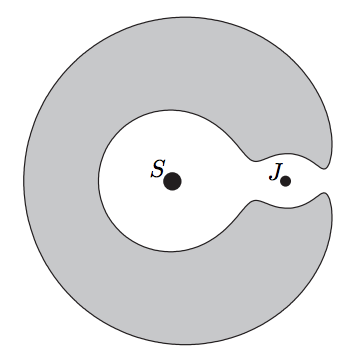
\includegraphics[scale=0.80]{fig/2bp-b_forbidden.png}
            \label{fig:forbidden-regions}
        }
        \caption{Visualizations of the potential. For some constant mechanical energy, \ref{fig:forbidden-regions} shows the allowed regions in white, forbidden in gray.}
    \label{fig:potential-visualizations}
\end{figure}
Looking at Figure \ref{fig:potential-visualizations}, we see that the lowest energy orbits must go through the saddle point or ``neck'' with the Lagrange point $L_1$ in the middle. However if we go straight to the Moon through the neck, we've seen that we arrive at the Moon with an excess velocity and must spend energy on breaking. Using a trajectory-search program to find trajectories through a region around $L_1$, we expect to find some Moon capture trajectories with lower delta-$v$ than Hohmann.
